\documentclass[aps,prb,twocolumn,amsfonts,showpacs,letterpaper]{revtex4}
\pdfoutput=1
\usepackage{amsmath}  % <- You need this package for 'align' environment
\usepackage{graphicx}  %<-  You need this package to insert graphics
\usepackage[nottoc]{tocbibind}
\usepackage{float}

\begin{document}
	\title{Diffusion Constant of 3D Random Walk}
	\author{John Rackham}
	\affiliation{Brigham Young University - Idaho: Physics 385 Student} 
	\date{\today} 

\maketitle

\section{Introduction}\label{intro}
Many real life systems include behavior that is random or unpredictable. One of the ways that effectively handles modeling these types of systems is the random walk method. A random walk is where a particle is said to move in a randomly determined direction of unity length, or of random lenth\cite{gio}. This work will examine a random walk in three dimensional space and determine the diffusion coefficient.

\section{Diffusion Coefficient}

\section{Results}

\begin{figure}[H]
\centering
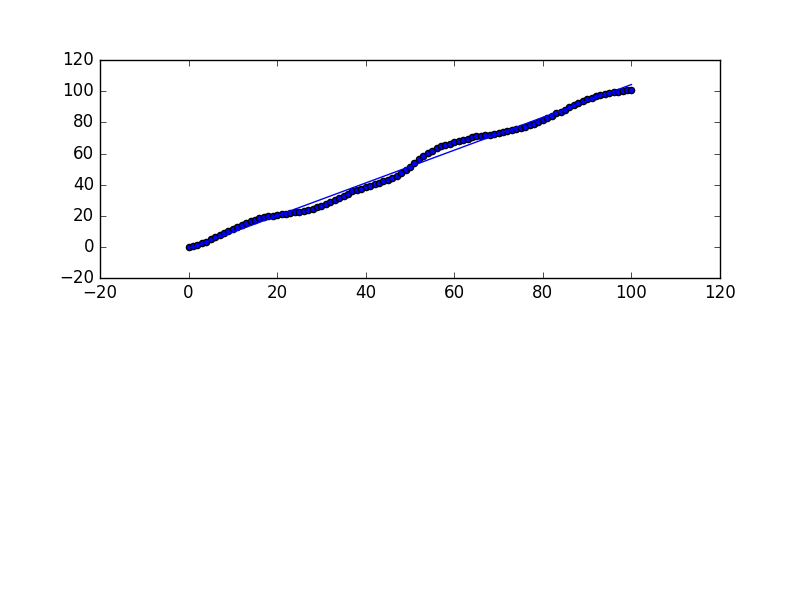
\includegraphics[scale=0.35]{figure_1.png}
\caption{cross section of the electric potential field}
\label{Voltage}
\end{figure}


\section{Conclusion}

\bibliography{refs}

\end{document}





